
\section{Design}
\subsection{Prototype overview}
Instead of having physical strings strung between the head and the bridge of the guitar, we employ Bela Trill Bar sensors. These will be positioned across the frets which will provide pressure-sensitive multi-touch to the guitar. A basic outline of the prototype can be seen in Figure \ref{fig:proposed}. In this prototype, the strings have been completely removed, and we will only employ the sensor input. This is an experimental design, but is intended to work as a forcing function \citep{norman_design_2013} to encourage exploration of the novel MPE features. Furthermore, strings may impact on the accuracy of the sensor data. 

This design is akin to the Chapman Stick k\citep{stick_enterprises_stick_2021}, and encourages two hands on the frets as as shown in Figure \ref{fig:chapman}.

\begin{figure}[h]
    \centering
    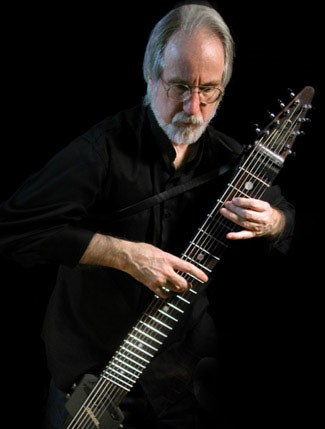
\includegraphics[scale=0.9]{Images/chapman.jpg}
    \caption{Chapman Stick style guitar, with a two-handed playing technique on the fretboard.}
    \label{fig:chapman}
\end{figure}

The prototype contains only six sensors in total, as any more is prohibitively expensive. The sensors occupy the 4th to 9th frets, as these are the frets which could accommodate the whole height of the Trill sensor. This means that on the frets which are occupied, all of the fret area is available to the user. 

The Bela Trill Bar sensors have a Grove connector on the back, so a small hole has been drilled through to neck to allow the wire to be passed through to the other side, so each sensor can be connected in series. Each of the sensors have also been trimmed to size to fit the appropriate width and height of their respective frets. 

With processing of the sensor data, this allows the array of sensors to act as if they were a matrix of fret-string locations, and thus can begin to emulate the behaviour of a traditional guitar.

Implementing the touch size and touch location data associated with each touch point will provide the data required to implement the MPE aftertouch and pitch bend functionality. 

The Bela Trill Bar sensors (Figure \ref{fig:trill_picture}) have been selected to play the central tole in this design for several reasons. Firstly, it affords multi-touch sensing, up to five simultaneous touches. which is sufficient for most guitar playing. 

It offers sensing in the horizontal direction only, but this is sufficient since notes are only differentiated horizontally on the guitar, and pitch bends (on traditional guitars) are also only available on this axis.

Secondly, it affords detection of touch size, which can be used as a proxy for pressure. Touch size and pressure are not the same, but are highly correlated. Therefore, we can use touch size in place of true pressure, and the prototype should offer a very similar behaviour compared to FSRs. In a more sophisticated prototype, we might consider incorporating additional sensors that can detect true pressure i.e. force sensitive resistors (FSRs). This would be beneficial as this would afford a more natural mapping between the gesture and the sound \citep{norman_design_2013}. This is because most acoustic instruments react to \textit{force} and not `touch size'. Therefore, a force-based interaction would represent an experience which is more representative of users experience with acoustic instruments which may be more successful overall. This is important as it links to \cite{norman_design_2013}'s 6th fundamental principal of design. Mapping in design, just like in mathematics, represents a connection between one set to another set. In this instance, the mapping of force exerted/touch size on the sensor, to the timbre (e.g. brightness) of the sound.  

\begin{figure}[h]
    \centering
    % 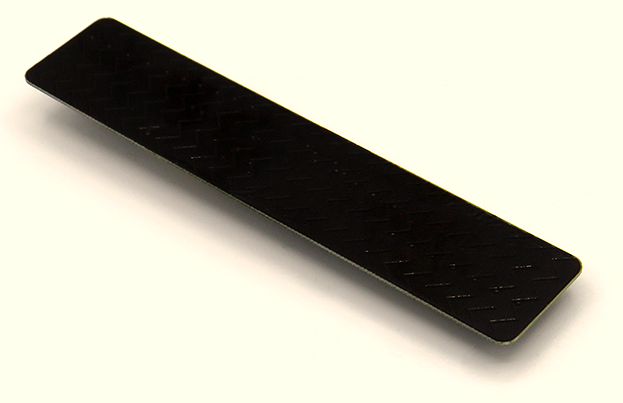
\includegraphics[scale=0.5]{Images/trill front.PNG}
    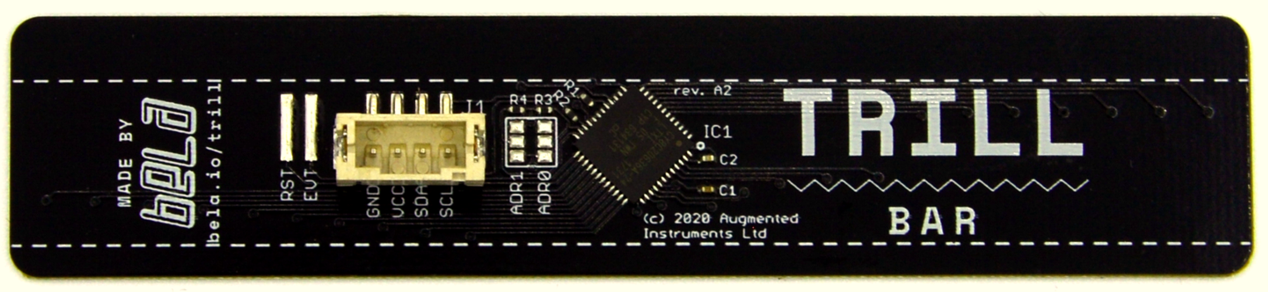
\includegraphics[scale=0.25]{Images/trill back.PNG}
    % \caption{Bela Trill Bar sensor front (top) and back (bottom). }
    \caption{Bela Trill Bar sensor. }
    \label{fig:trill_picture}
\end{figure}

In the design of this prototype, FSRs were also examined to be the principle sensor to comprise this design. As stated above, these do come with the added benefit of \textit{true} force sensing, not just using touch size as a proxy, which may result in a more expressive final product, but they also come with more drawbacks. 

However, this would only support pressure detection, and not pitch bending, since we would not be able to detect the continuous horizontal variance across the width of the frets which is essential for pitch bending. 

Furthermore, this would require a very large amount of analogue inputs into the micro-controller (one per fret-string location), which would rapidly be exhausted, as the number of frets supported increased. 

In future iterations of the design this could offer additional information on top of the capacitive sensors, which could make the instrument more expressive. 

\begin{figure}
    \centering
    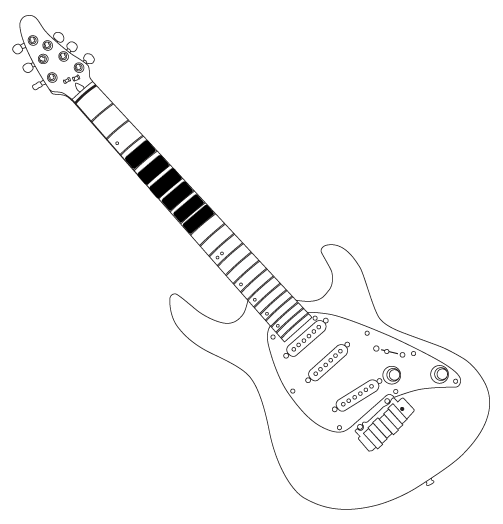
\includegraphics[scale=0.65]{Images/NEWGUITA.png}
    \caption{Basic prototype design}
    \label{fig:proposed}
\end{figure}

\begin{figure*}
    \centering
    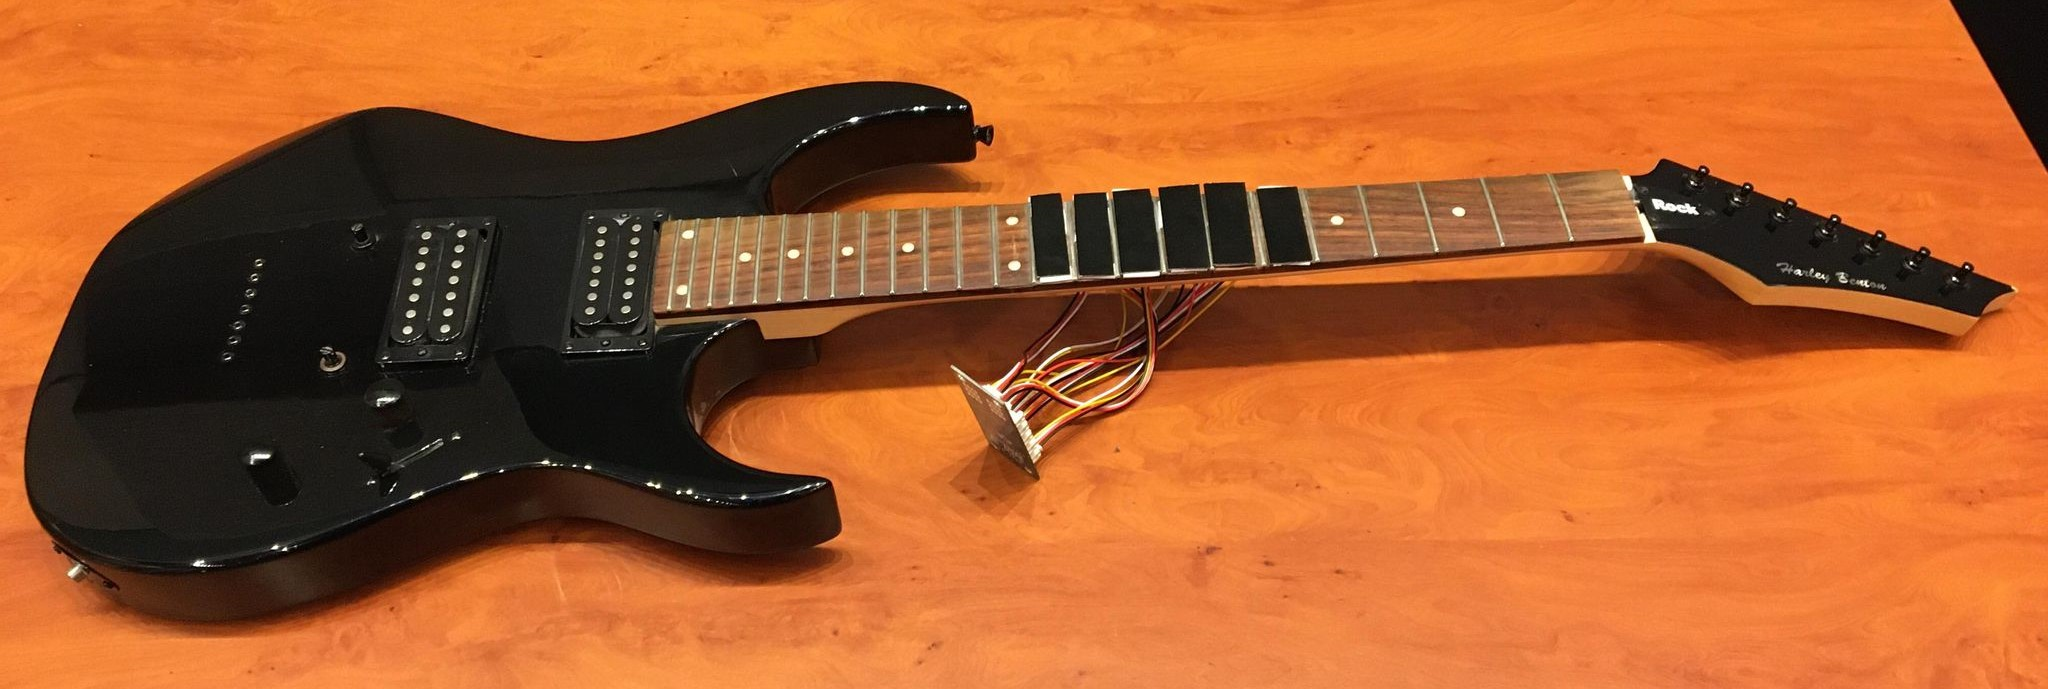
\includegraphics[scale=0.33]{Images/guitar1.jpg}
    \caption{Final prototype. See Appendix \ref{appendices:guitarimages} for more images of the final prototype.}
    \label{fig:guitarfront1}
\end{figure*}


% =========================================
\section{Software Implementation}

\subsection{Sensor to MIDI Translation}
We can summarise the logical overview of sensor input to MIDI instructions with the diagram shown in Figure \ref{fig:logicFlow}.
\subsubsection{Sensor discretisation \& touch identification}

\begin{figure}
    \centering
    \begin{tikzpicture}
 [node distance=4.35cm]
\node (n1)[rectangle,draw]at (0,0) {1) Sensor discretisation \& touch identification};
\node (n2)[rectangle,draw] at ($(n1.south)+(0.0,-1.0)$) {2) Populate touch matrix from activations of sensors};
\node (n3)[rectangle,draw] at ($(n2.south)+(0.0,-1.0)$) {3) Determine note onsets \& offsets};
\node (n4)[rectangle,draw] at ($(n3.south)+(0.0,-1.0)$) {4) Generate MIDI note-on and note-off events};
\node (n5)[rectangle,draw] at ($(n4.south)+(0.0,-1.0)$) {5) Assign events to relevant MIDI channels};
\node (n6)[rectangle,draw] at ($(n5.south)+(0.0,-1.0)$) {6) Execute MIDI from Note Event List};

% Connectors
\draw [-latex] (n1) -- (n2);
\draw [-latex] (n2) -- (n3);
\draw [-latex] (n3) -- (n4);
\draw [-latex] (n4) -- (n5);
\draw [-latex] (n5) -- (n6);

\end{tikzpicture}
    \caption{Logical overview of the sensor data to MIDI event conversion.}
    \label{fig:logicFlow}
\end{figure}

Each fret of the system is represented by a Bela Trill Bar sensor, which has continuous expression in the horizontal axis.

We are then faced with the challenge of discretizing this continuous dimension into 'string zones', such that, if there are 6 strings (which is the case for the traditional guitar), all touches within the first sixth of the bar are categorized as string $0$, all touches within the second sixth of the bar are categorized as string $1$, and so on. 

Trill sensor data is already normalized to the range of $0$ to $1$, which means that the far 'left' of the sensor represents a mapping of $X$ to $0$, and the far right represents where $X$ maps to $1$.

Using this knowledge and knowing how many strings we want to use in the system we can determine the width and boundary locations of each string zone. Expression \ref{eq:string-boundaries} describes the set of string boundaries $\mathbf{B}$, which has length  $L$ and where $S$ is the number of strings.
\begin{equation} \label{eq:string-boundaries}
\mathbf{B}_n = \frac{n}{L}, \: \: \: \: \: \: \: \: n \in [0:S-1], \; \; \;  n \in \mathbb{Z}
\end{equation}

It is recognised that $S + 1$ boundaries are typically required to delineate a region completely, however, since we are bound to not receive input over $1.0$, this `implies' our final upper bound. We can use this fact to reduce the complexity of our program.

Having discretized all touches into string zones, and knowing their fret index, we can construct a binary matrix that represents touches on each fret-string location. This is required to determine note onset and offsets, which does not directly relate to the MPE behaviour of the system, but is a necessary pre-requisite for all MIDI instruments.


\newcommand{\trillWidth}{101.6mm / 1.2}
\newcommand{\trillHeight}{21.5mm / 1.2}
\newcommand{\NumStrings}{6}
\newcommand{\StringWidth}{\trillWidth/\NumStrings}
\begin{figure}[h]
    \centering
    \begin{tikzpicture}
    \usetikzlibrary{shapes.misc, positioning, svg.path}
    
    \fill [black,draw]
  {[rounded corners=6](0,0) --
  ++(\trillWidth, 0)  --
  ++(0, \trillHeight) --
  ++(-\trillWidth, 0) --
  cycle
  {}};

  \draw[white, thick, dashed] (0, 0) -- (0 ,\trillHeight);
  \draw[white, thick, dashed] (\StringWidth*1, 0) -- (\StringWidth*1 ,\trillHeight);
  \draw[white, thick, dashed] (\StringWidth*2, 0) -- (\StringWidth*2 ,\trillHeight);
  \draw[white, thick, dashed] (\StringWidth*3, 0) -- (\StringWidth*3 ,\trillHeight);
  \draw[white, thick, dashed] (\StringWidth*4, 0) -- (\StringWidth*4 ,\trillHeight);
  \draw[white, thick, dashed] (\StringWidth*5, 0) -- (\StringWidth*5 ,\trillHeight);
  
   %\draw[white, thick, dashed] (0, 0) -- (0 ,\trillHeight);
   \node[align=left] at (\StringWidth*0, -0.3) {0.0};
   \node[align=left] at (\StringWidth*1, -0.3) {0.16};
   \node[align=left] at (\StringWidth*2, -0.3) {0.33};
   \node[align=left] at (\StringWidth*3, -0.3) {0.50};
   \node[align=left] at (\StringWidth*4, -0.3) {0.66};
   \node[align=left] at (\StringWidth*5, -0.3) {0.83};
   
   \node[draw,circle, fill=red, text=white] at (\StringWidth/2 + \StringWidth*2,\trillHeight/2) {0.40};

    \end{tikzpicture}
    \caption{Demonstration of the sensor boundaries $\mathbf{B}_n$ for N=6. The vertical dashed lines represent the string boundaries $\mathbf{B}_n$, \textit{not} digital strings. }
    \label{fig:my_label}
\end{figure}

We can determine the string zone of the red dot with the following logic, shown is pseudo-code in Figure \ref{fig:getStringZone}. 
\begin{figure}[h]
    \centering
    \begin{verbatim}
int getStringZone(float touchLocation)
{
    for i=0:length(Bn):
        if(touchLocation >= Sn[i]):
            return i
    return -1 // Error, out of range. 
}
\end{verbatim}
    \caption{String zone determining algorithm pseudo-code.}
    \label{fig:getStringZone}
\end{figure}


Which will return $\mathbf{B}_n = 2$ for $S=6$. 

\subsubsection{Populate touch matrix from activations of sensors}
Since we know the index of each sensor, we can construct a strings $\times$ frets matrix like so. For example with three sensors, as is shown in Figure \ref{fig:trill_touches}, we can generate the binary matrix in Figure \ref{fig:binary_matrix}.

Here, we will also define the notation for discussing each individual cells of the matrix diagrams. In Figure \ref{fig:binary_matrix}, the $\mathbf{1}$ in the top row would have position $(0, 3)$, the middle row $(1, 0)$ and the bottom row $(2, 5)$. Fret index increases with vertical movement down, and string index increases with horizontal movement to the right. 


% \newcommand{\trillWidth}{101.6mm / 1.2}
% \newcommand{\trillHeight}{21.5mm / 1.2}
% \newcommand{\NumStrings}{6}
% \newcommand{\StringWidth}{\trillWidth/\NumStrings}
\begin{figure}[h]
    \centering
    \begin{tikzpicture}
    \usetikzlibrary{shapes.misc, positioning, svg.path}
    
    \fill [black,draw]
  {[rounded corners=6](0,0) --
  ++(\trillWidth, 0)  --
  ++(0, \trillHeight) --
  ++(-\trillWidth, 0) --
  cycle
  {}};
  \draw[white, thick, dashed] (0, 0) -- (0 ,\trillHeight);
  \draw[white, thick, dashed] (\StringWidth*1, 0) -- (\StringWidth*1 ,\trillHeight);
  \draw[white, thick, dashed] (\StringWidth*2, 0) -- (\StringWidth*2 ,\trillHeight);
  \draw[white, thick, dashed] (\StringWidth*3, 0) -- (\StringWidth*3 ,\trillHeight);
  \draw[white, thick, dashed] (\StringWidth*4, 0) -- (\StringWidth*4 ,\trillHeight);
  \draw[white, thick, dashed] (\StringWidth*5, 0) -- (\StringWidth*5 ,\trillHeight);
   
   \node[draw,circle, fill=red, text=white] at (\StringWidth/2 + \StringWidth*3,\trillHeight/2) {0.63};
    \end{tikzpicture}
    
     \centering
    \begin{tikzpicture}
    \usetikzlibrary{shapes.misc, positioning, svg.path}
    
    \fill [black,draw]
  {[rounded corners=6](0,0) --
  ++(\trillWidth, 0)  --
  ++(0, \trillHeight) --
  ++(-\trillWidth, 0) --
  cycle
  {}};
  \draw[white, thick, dashed] (0, 0) -- (0 ,\trillHeight);
  \draw[white, thick, dashed] (\StringWidth*1, 0) -- (\StringWidth*1 ,\trillHeight);
  \draw[white, thick, dashed] (\StringWidth*2, 0) -- (\StringWidth*2 ,\trillHeight);
  \draw[white, thick, dashed] (\StringWidth*3, 0) -- (\StringWidth*3 ,\trillHeight);
  \draw[white, thick, dashed] (\StringWidth*4, 0) -- (\StringWidth*4 ,\trillHeight);
  \draw[white, thick, dashed] (\StringWidth*5, 0) -- (\StringWidth*5 ,\trillHeight);
   
   \node[draw,circle, fill=red, text=white] at (\StringWidth/2 + \StringWidth*0,\trillHeight/2) {0.08};
   
    \end{tikzpicture}
    
     \centering
    \begin{tikzpicture}
    \usetikzlibrary{shapes.misc, positioning, svg.path}
    
    \fill [black,draw]
  {[rounded corners=6](0,0) --
  ++(\trillWidth, 0)  --
  ++(0, \trillHeight) --
  ++(-\trillWidth, 0) --
  cycle
  {}};
  \draw[white, thick, dashed] (0, 0) -- (0 ,\trillHeight);
  \draw[white, thick, dashed] (\StringWidth*1, 0) -- (\StringWidth*1 ,\trillHeight);
  \draw[white, thick, dashed] (\StringWidth*2, 0) -- (\StringWidth*2 ,\trillHeight);
  \draw[white, thick, dashed] (\StringWidth*3, 0) -- (\StringWidth*3 ,\trillHeight);
  \draw[white, thick, dashed] (\StringWidth*4, 0) -- (\StringWidth*4 ,\trillHeight);
  \draw[white, thick, dashed] (\StringWidth*5, 0) -- (\StringWidth*5 ,\trillHeight);
   
   \node[draw,circle, fill=red, text=white] at (\StringWidth/2 + \StringWidth*5,\trillHeight/2) {0.91};
   
    \end{tikzpicture}
    
    \caption{Example of sensors with touch locations in the relevant string zones. The vertical dashed lines represent the string boundaries $\mathbf{B}_n$, \textit{not} digital strings. }
    \label{fig:trill_touches}
\end{figure}

\begin{figure}[h]
    \centering
    \begin{tikzpicture}
    \matrix (mD) [draw,matrix of math nodes]
    {
    0 & 0 & 0 & \textbf{1} & 0 & 0 \\
    \textbf{1} & 0 & 0 & 0 & 0 & 0 \\
    0 & 0 & 0 & 0 & 0 & \textbf{1} \\
    };
    
    \node[rotate=90] at (-1.8cm, 0) {Fret Index};
    \node at (-0.0cm, 1.2cm) {String Index};
    
    \end{tikzpicture}
    \caption{Binary matrix interpreted from sensor positions.}
    \label{fig:binary_matrix}
\end{figure}

\subsubsection{Determine note onsets \& offsets}
Note-on and note-off events are not trivial to detect as they can only be determined \textit{between} audio callbacks, not \textit{within}. Meaning, that no single `snapshot' of a touch matrix is sufficient to determine note onsets or offsets. This means that there must be a system for `remembering' which fret-string locations were active in the previous audio callbacks. 

This is achieved by the comparison of a \textit{pair} of binary matrices,  where each element represents a logical Boolean value. One matrix, $\mathbf{C}$, represents the \textbf{c}urrent activation (presence of touch) of fret-string locations in the audio callback and one matrix, $\mathbf{P}$, which represents activations in the \textbf{p}revious audio callback.

To determine note onsets, we can perform the following element-wise logical operation on $\mathbf{C}$ and $\mathbf{P}$, which will generate a third binary matrix,  $\mathbf{Onsets}$, which represents the position of note onsets. 
\begin{equation} \label{eq:onsets}
\begin{aligned}
\mathbf{Onsets}_{f,s} := \mathbf{C}_{f,s} \land \lnot \mathbf{P}_{f,s}, \\
 f \in [0:F-1],  \: \:  s \in [0:S-1]
\end{aligned}
\end{equation}

Where $F$ is the number of `frets' and $S$ is the number of `strings'. 

What follows is the matching expression for the note off binary matrix, $\mathbf{Offsets}$. 

\begin{equation} \label{eq:offsets}
\begin{aligned}
\mathbf{Offsets}_{f,s} := \lnot \mathbf{C}_{f,s} \land \mathbf{P}_{f,s}, \\
 f \in [0:F-1],  \: \:  s \in [0:S-1]
\end{aligned}
\end{equation}

This is visually expressed with a simplified example in Figure \ref{fig:fret-matrix}.
\begin{figure}[h]
\centering
\begin{tikzpicture}[every node/.style={anchor=north east, fill=white, minimum width=0.5cm, minimum height=5mm}]

% OFFSETS
\matrix (mA) [draw,matrix of math nodes]
{
0 & 0 & 0 & 0 & 0 & 0 \\
0 & 0 & 0 & 0 & 0 & 0 \\
0 & 0 & 0 & \mathbf{1} & 0 & 0 \\
0 & 0 & 0 & 0 & 0 & 0 \\
};

% ONSETS
\matrix (mB) [draw,matrix of math nodes] at ($(mA.south west)+(1.5,0.7)$)
{
\mathbf{1} & 0 & 0 & 0 & 0 & 0 \\
0 & 0 & 0 & 0 & 0 & 0 \\
0 & 0 & 0 & 0 & 0 & 0 \\
0 & 0 & 0 & 0 & 0 & 0 \\
};

% C
\matrix (mC) [draw,matrix of math nodes] at ($(mB.south west)+(1.5,0.7)$)
{
\mathbf{1} & 0 & 0 & 0 & 0 & 0 \\
0 & 0 & 0 & 0 & 0 & 0 \\
0 & 0 & 0 & 0 & 0 & 0 \\
0 & 0 & 0 & 0 & 0 & 0 \\
};

% P
\matrix (mD) [draw,matrix of math nodes] at ($(mC.south west)+(1.5,0.7)$)
{
0 & 0 & 0 & 0 & 0 & 0 \\
0 & 0 & 0 & 0 & 0 & 0 \\
0 & 0 & 0 & \mathbf{1} & 0 & 0 \\
0 & 0 & 0 & 0 & 0 & 0 \\
};

\node[align=left] at ($(mD.south east) + (-0.1cm, -0cm)$){$\mathbf{P}$};
\node[align=left] at ($(mC.south east) + (-0.4cm, -0cm)$) {$\mathbf{C}$};
\node[align=left] at ($(mB.south east) + (-0.3cm, -0cm)$) {$\mathbf{Onsets}$};
\node[align=left] at ($(mA.south east) + (-0.3cm, -0cm)$) {$\mathbf{Offsets}$};

\draw[latex-, dashed](mA.north east)--(mD.north east);
\draw[latex-, dashed](mA.north west)--(mD.north west);
\draw[latex-, dashed](mA.south east)--(mD.south east);
\end{tikzpicture}

\caption{Demonstration of binary matrix operation for onsets and offsets using the expressions \ref{eq:onsets} and \ref{eq:offsets}}
\label{fig:fret-matrix}

\end{figure}

\subsubsection{Generate MIDI note-on and note-off events}

At this point it is possible to convert fret-string locations to MIDI number, and send the required MIDI note-on and note-off instructions. However, this presents us with a problem that is unique to guitar-style MIDI controllers.

We must convert the $\mathbf{Onsets}$ and $\mathbf{Offsets}$ into MIDI instructions so that our prototype can communicate with digital instruments and DAWs in a format that is understood.

Furthermore, we must `remember' which notes are currently \textit{active} (have had an onset, but hasn't yet had an offset), and to ensure that all \textit{active} notes are correctly terminated at the appropriate time. Failing to do this will result in notes that do not correctly stop at the right time, creating a cacophonous barrage of notes which will ultimately be frustrating for the user.

This requires that each fret-string location is individually addressable, such that when location $(0, 1)$ has an onset corresponding to MIDI note $45$, for example, when that corresponding offset is sent, that note is in fact terminated.

We might be tempted to use MIDI notes as the identifier for fret-string locations such that when $(0, 1)$ is played we store in memory that note $45$ is currently active, and when we receive the corresponding offset that matches up with MIDI note $45$, we terminate that note. This logic would work fine for a piano or keyboard MIDI controller, because each key has a \textit{unique} mapping to any given MIDI note. This is not the case with the guitar. Figure \ref{fig:midicantormatrix}a shows the mapping of fret-string locations to MIDI note number for standard EADGBE guitar tuning.

\newcommand{\higl}[1]{\textit{\textbf{#1}}}
\begin{figure}[h]
    \centering
    \begin{tikzpicture}
    \matrix (midi) [draw,matrix of math nodes]
    {
    40 & \higl{45} & \higl{50} & \higl{55} & \higl{59} & \higl{64} \\
    41 & \higl{46} & \higl{51} & \higl{56} & \higl{60} & \higl{65} \\
    42 & 47 & 52 & 57 & 61 & 66 \\
    43 & 48 & 53 & 58 & 62 & 67 \\
    44 & 49 & 54 & 59 & 63 & 68 \\
    \higl{45} & \higl{50} & \higl{55} & \higl{60} & \higl{64} & 69 \\
    \higl{46} & \higl{51} & \higl{56} & \higl{61} & \higl{65} & 70 \\
    };
    
    \matrix (cantor) [draw,matrix of math nodes] at ($(midi.east)+(2.3, 0.0)$)
    {
    0&	1&	3&	6&	10&	15& \\
    2&	4&	7&	11&	16&	22&\\
    5&	8&	12&	17&	23&	30&\\
    9&	13&	18&	24&	31&	39&\\
    14&	19&	25&	32&	40&	49&\\
    20&	26&	33&	41&	50&	60&\\
    27&	34&	42&	51&	61&	72&\\
    };
    
    \node[rotate=90] at (-2.3cm, 0) {Fret Index};
    \node at (-0.0cm, 2.1cm) {a. String Index (MIDI)};
    \node at (4.2cm, 2.1cm)  {b. String Index (Cantor)};
    
    \end{tikzpicture}
    \caption{Demonstration that there are not unique mappings from fret-string locations to MIDI notes, which therefore cannot be used as unique identifiers for notes. Highlighted numbers are non-unique. Diagram represent the first seven frets. }
    \label{fig:midicantormatrix}
\end{figure}

It can clearly be seen that there are MIDI note duplicates in this matrix, which means that there is not a unique mapping of fret-string locations to MIDI notes. This means that a user might press $(0, 1)$ for example, and then presses $(5, 0)$, this would override the former, and both notes would be terminated if either touch were released. 

This behaviour is not analogous to any typical acoustic instrument, and is therefore unlikely to match up with user's expectations. This unexpected behaviour is not only likely to disturb the user's workflow, but is also limits the possible actions of the user, which may not be conducive to their creativity.

% This behaviour is unlikely to match up with user's expectations in an unpleasing way, as they would expect independent behaviour for notes. 

Therefore, we require another method for uniquely identifying fret-string locations. For this we can use the Cantor pairing algorithm. This expression creates an ordered mapping between all pairs of natural numbers to the set of natural numbers. The expression for a two-element Cantor pairing is defined as so:

\begin{equation} \label{eq:cantor}
    \pi(k_1, k_2) := \frac{1}{2}(k_1 + k_2)(k_1 + k_2 + 1) + k_2
\end{equation}


\tikzset{->-/.style={decoration={
  markings,
  mark=at position #1 with {\arrow{>}}},postaction={decorate}}}
  
\begin{figure}[h]
    \centering
    
    \begin{tikzpicture}[scale=2.2]
    \clip(-0.60,-0.60) rectangle (3.40,3.45);
    \tkzInit[xmax=4,ymax=4,xmin=0,ymin=0]
    \tkzGrid
    \tkzAxeXY
    \node at (1.75, -0.5){\large $k_1$};
    \node[] at (-0.5, 1.75){\large $k_2$};
    
    % Draws the first blue line and red circle.
    \draw[thick,->-=.5,blue] (0,0) -- (1,0);
    \filldraw (0,0)[red] circle (1.7pt);
    
    % <THIS DRAWS THE BLUE LINES>
    \newcounter{N}{0}
    \foreach \n in {1,...,15} {
        \foreach \i in {0,...,\value{N}}{
            \draw[thick, ->-=.5,blue] (\n - \i, \i) -- (\n - 1 - \i ,\i + 1);
        }
        \stepcounter{N}
        \draw[thick, ->-=.5,blue] (0,\n) -- (\n+1,0); %IMPORTANT
    } % END <THIS DRAWS THE BLUE LINES>
    
    % <THIS DRAWS THE NUMBER AND RED DOTS>
    % These are 'registers' used to calculate the cantor number. 
    \setcounter{N}{3}
    \newcounter{cn}{0}
    \newcounter{r1}{0}
    \newcounter{r2}{0}
    \newcounter{r3}{0}
    \foreach \n in {0,...,3} {
        \foreach \i in {0,...,\value{N}}{
            % Fill circles. 
            \filldraw (\i, \n)[red] circle (1.5pt);
            
            %% CALCULATE CANTOR NUMBER
            % Reset registers. 
            \setcounter{cn}{0}
            \setcounter{r1}{\i}
            \setcounter{r2}{\n}
            \setcounter{r3}{0}
            
            % cn = (k1 + k2 + 1)
            \addtocounter{cn}{\value{r1}}
            \addtocounter{cn}{\value{r2}}
            \addtocounter{cn}{1}
            
            % r3 = (k1 + k2)
            \addtocounter{r3}{\value{r1}}
            \addtocounter{r3}{\value{r2}}
            
            % cn *= r3
            \multiply\value{cn} by \value{r3}
            
            % cn /= 2
            \divide\value{cn} by 2
            
            % cn += k2
            \addtocounter{cn}{\value{r2}}
            %% END CALCULATE CANTOR NUMBER
            
            % Display cantor number. 
            \node at (\i + 0.125, \n + 0.125){\arabic{cn}};
        }
    } % END <THIS DRAWS THE NUMBERS AND RED DOTS>
   
\end{tikzpicture}
    \caption{Visualization of the two element Cantor pairing algorithm.}
    \label{fig:my_label}
\end{figure}



Which means that each fret-string location can now be uniquely identified by a single integer. This means that we can now easily distinguish note events which have identical MIDI note values. We can compare the identifier numbers for each fret-string location by looking at Figure \ref{fig:midicantormatrix}. Note that in Figure \ref{fig:midicantormatrix}b that there is no duplication in any of the cells of the matrix. 

\subsubsection{Assign events to relevant MIDI channels}
Furthermore, to create MPE behaviour, we must be able to assign notes uniquely to MIDI channels in an efficient way. The MIDI 1.0 Protocol works in such a way that each MIDI \textit{channel} has pitch-bend and aftertouch, not each \textit{note}. This means that every note on any given channel would all be equally detuned by the same pitch bend instruction. This is typically very unmusical because very few acoustic instruments exhibit behaviour like this. 

This is the motivation to implement MPE behaviour, where each note is assigned to its own channel and thus had independent pitch-bend and after-touch, making for a more expressive instrument. 

However this represents a more complex programming task in both the controller/sensor design and the software instrument design. 
We must remember which notes, or indeed fret-string hashes as determined by expression \ref{eq:cantor}, are currently active. Furthermore, we must free MIDI channels as notes receive their offsets, such that we always choose the lowest index MIDI channel as possible. There are only 16 in total, and wish to avoid sending an invalid MIDI instructions, which may crash either one of the controller or MIDI host, which will prevent the user from working.

To complete this task we can create a length 16 list of `active notes'. Which represents the maximum number of MIDI channels and the maximum number of possible simultaneous notes playable on this controller. This limit is very likely to be sufficient, a maximum of 6 notes are expected (one per string) and a theoretical maximum of 10 notes are playable (one per finger), though the latter would represent a rather experimental technique. 

To create the behaviour required, we require multiple data points about each note event, and thus the list (implemented with a C++ standard library \texttt{vector}) is populated with the data structure shown in Figure \ref{fig:noteevent}.
\begin{figure}[h]
\begin{mdframed}
    \begin{verbnobox}[\small]
struct NoteEvent
{
    	int midiNote = -1;
    	int midiChannel = -1;
    	int velocity = -1;
    	int pressure = -1;
    	int pitchBend = -1;
    	float initialTouchLocation = -1;
    	int fretStringHash = -1;
    	bool isActive = false;
    	bool dueOnset  = false;
    	bool dueOffset = false;
};
    \end{verbnobox}
    \end{mdframed}
        \caption{\texttt{NoteEvent} data structure.}
    \label{fig:noteevent}
\end{figure}

In this data structure there are some other elements which will be discussed in later sections about MIDI continuous control (CC) instructions.

We can use this list of \texttt{NoteEvents} in order to describe which note events should be executed.

When a new note onset is detected, we can determine which element in the list it should occupy with the algorithm described in Figure \ref{fig:noteon}. This algorithm ensures that the selected index in the \texttt{noteEventList} is as small as possible. 

\begin{figure}[H]
\begin{mdframed}
\begin{verbnobox}[\small]
let noteEventList = vector<NoteEvent>{16}
let newOnset = {fret, str, ...}

for i=0:length(noteEventData)-1:
{
    if(!noteEventData[i].isActive)
    {
         noteEventData[i] = newOnset
         noteEventData[i].dueOnset = true
         noteEventData[i].isActive = true
    }
}
\end{verbnobox}
\end{mdframed}
\caption{Pseudo-code algorithm for determining the index of and creating new \texttt{NoteEvent} objects.}
\label{fig:noteon}
\end{figure}

Conversely, when a note offset is detected, and stated in the $\mathbf{Offsets}$ matrix, we can perform the following algorithm to edit the \texttt{noteEventList}.


\begin{figure}[h]
\begin{mdframed}
\begin{verbnobox}[\small]
let noteEventList = vector<NoteEvent>{16}
let newOnset = {fret, str, ...}

for i=0:length(midiList)-1:
{
    if(noteList[i].fsHash==cPair(fret,str))
    {
         noteList[i].isDueNoteOffset = true
    }
}
\end{verbnobox}
    \end{mdframed}
        \caption{Pseudo-code to mark \texttt{NoteEvent}s as ready to recieve a MIDI note off event.}
    \label{fig:noteoff}
\end{figure}

Conveniently, we can use the indices of the \texttt{NoteEvent} list to determine the MIDI channel for each note, as they are always the lowest value possible for a given note, and unique to each note. This is the case because as we can see in line 5 of Figure \ref{fig:noteon} as we iterate over \texttt{i}, we will `stop' at the lowest value of \texttt{i} that does not contain an active note and assign it the new note. 

\subsubsection{Execute MIDI from Note Event List}
Now we have a list of which MIDI notes to turn on and off, appropriately matched to a channel such that we can take advantage of MPE style behaviour.

This can be done by the C++ function in Figure \ref{fig:write_midi_function}, which implements the Bela MIDI API.

\begin{figure}[h]
\begin{mdframed}
\begin{lstlisting}
#define CH0_NOTE_ON  144
#define CH0_NOTE_OFF 128
using Midi = midi_byte_t;
void writeNote(int event, // 0->ON, 1->OFF
               int ch,    // midi channel
               Midi note, // note number
               Midi vel = 0) // velocity 
{
    int eventType = (event == 0)
            ? CH0_NOTE_ON : CH0_NOTE_OFF;
    Midi status =  Midi(eventType + ch);
    Midi out[3] = {status, note, vel};
    midi.writeOutput(out, 3);
}
\end{lstlisting}
\end{mdframed}
        \caption{C++ code using the Bela MIDI API to send note-on and note-off instructions.}
    \label{fig:noteoff}
\end{figure}

We then need to iterate though all elements of \texttt{NoteEvent}s and perform the proper function, which can be implemented with the code outlined in Figure \ref{fig:write_midi_function}.

\begin{figure*}[h]
\begin{mdframed}
\begin{lstlisting}
void writeMidiFromNoteEvents()
{
    for(int i = 0; i < gNoteEventData.size(); i++)
    {
        if(gNoteEventData[i].isActive)
        {
            if(gNoteEventData[i].isDueNoteOffset)
            {
                writeNote(1, i, gNoteEventData[i].midiNote);
                gNoteEventData[i].isDueNoteOffset = false;
                gNoteEventData[i].isActive = false;
            }
			
            if(gNoteEventData[i].isDueNoteOnset)
            {
                gNoteEventData[i].isDueNoteOnset = false;
                writeNote(0, i, gNoteEventData[i].midiNote, gNoteEventData[i].velocity);
            }
				
            writeAftertouch(i, gNoteEventData[i].pressure);
            midi.writePitchBend((midi_byte_t)i, gNoteEventData[i].pitchBend);
        }
    }
}
\end{lstlisting}
\end{mdframed}
    \caption{C++ code using the Bela MIDI API to send note-on and note-off instructions.}
    \label{fig:write_midi_function}
\end{figure*}

%TODO FINISH THIS SECTION

\subsection{MPE Aftertouch and Pitchbend}

Currently, we have only discussed how to implement basic note onsets and note offsets. While necessary, this is not sufficient to meet our requirement to implement MPE style behaviour. In order to create a compelling MPE experience, it is typical to implement aftertouch and pitch bend functionality. 

\textbf{Aftertouch} typically is an expression of `pressure' which can be expressed \textit{after} the onset of the note. It is typically used to map a force/pressure on a key to a note's amplitude or timbre. This might be likened to a saxophonist who may start a note by breathing quietly, and then crescendo the amplitude of the note before its offset. As stated above, force from an FSR would possibly make a more appropriate input for this parameter, however we are limited by the capabilities of the Bela Trill sensors, which can only interpret touch size. However, this does serve as a very reasonable proxy for force/pressure.

Since the acoustic and electric guitar is a plucked/strummed instrument, this type of expression is typically not available. This attempt to extend the expressive capacity of the guitar or guitar-like instruments is central to the motivation of this study.

\textbf{Pitchbend} is a feature which is typically implemented by a wheel to the left of the keys on standard MIDI keyboards (see Figure \ref{fig:pitchwheel}).

\begin{figure}[h]
    \centering
    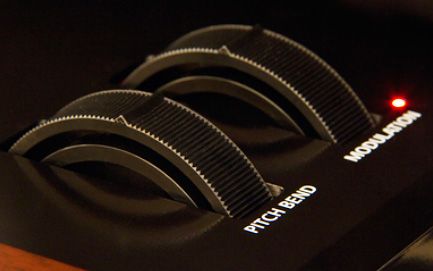
\includegraphics[scale=0.5]{Images/pitch bend.jpg}
    \caption{Typical pitch bend wheel}
    \label{fig:pitchwheel}
\end{figure}

However since we would like to emulate the expressive bending of guitar strings with this design, we must convert the touch location data into meaningful MIDI pitchbend data.s

These features can be implemented by a simple extension of the framework laid out above. In our basic touch matrices shown in Figures \ref{fig:binary_matrix} and \ref{fig:fret-matrix}, we store only a single Boolean value. Instead, we could store a more complex data structure which will help implement our MPE behaviour based on other sensor data such touch size and touch location. 

For each touch on each sensor, we must collect three important pieces of information. 

\begin{itemize}
    \item \texttt{bool isActive}: Whether this location in the fret-string matrix currently has a touch present.
    \item \texttt{float touchSize}: The size of the touch. This is a proxy for pressure, and can be used to implement our aftertouch functionality. 
    \item \texttt{float touchLocation}: The precise location on the sensor where the touch currently is.  
\end{itemize}

Now, each matrix $\mathbf{C}$ and $\mathbf{P}$ can be considered a 3D data structure, which would represent the arrangement of touches shown in Figure \ref{fig:trill_touches} in the following diagram, Figure \ref{fig:new_struct}. This assumes all touch sizes are 0.5 for simplicity, however this is entirely variable between 0 and 1. 

\begin{figure}[h]
\centering
\begin{tikzpicture}[every node/.style={anchor=north east, fill=white, minimum width=0.5cm, minimum height=5mm}]



% OFFSETS
\matrix (mA) [draw,matrix of math nodes]
{
0.00 & 0.00 & 0.00 & \textbf{0.63} & 0.00 & 0.00 \\
\textbf{0.08} & 0.00 & 0.00 & 0.00 & 0.00 & 0.00 \\
0.00 & 0.00 & 0.00 & 0.00 & 0.00 & \textbf{0.91} \\
};

% ONSETS
\matrix (mB) [draw,matrix of math nodes] at ($(mA.south west)+(2.9,0.7)$)
{
0.00 & 0.00 & 0.00 & \textbf{0.50} & 0.00 & 0.00 \\
\textbf{0.50} & 0.00 & 0.00 & 0.00 & 0.00 & 0.00 \\
0.00 & 0.00 & 0.00 & 0.00 & 0.00 & \textbf{0.50} \\
};

% C
\matrix (mC) [draw,matrix of math nodes] at ($(mB.south west)+(2.5,0.7)$)
{
0 & 0 & 0 & \textbf{1} & 0 & 0 \\
\textbf{1} & 0 & 0 & 0 & 0 & 0 \\
0 & 0 & 0 & 0 & 0 & \textbf{1} \\
};

\node[align=left] at ($(mC.south east) + (-0.4cm, -0cm)$) {\texttt{isActive}};
\node[align=left] at ($(mB.south east) + (-0.5cm, -0cm)$) {\texttt{touchSize}};
\node[align=left] at ($(mA.south east) + (0.6cm, -0cm)$) {\texttt{touchLocation}};
\end{tikzpicture}

\caption{A visual representation of the updated data structure used to represent touch information. }
\label{fig:new_struct}

\end{figure}
 
In the case of aftertouch, all that must be done is to look up the fret-string/Cantor hash of the given location, scale the touch size to the given aftertouch range as specified by the MIDI 1.0 documentation, and write the result to the output as per Figure \ref{fig:write_midi_function}. This scaling can be achieved by the following means:

\DeclarePairedDelimiter\ceil{\lceil}{\rceil}
\DeclarePairedDelimiter\floor{\lfloor}{\rfloor}
\begin{equation}
    y = \floor{x \cdot AT_{max}}
    \label{eq:scaling}
\end{equation}

Where $AT_{max}$ is the maximum valid aftertouch value. This expression can also be used with maximum velocity $V_{max}$ to give meaningful and valid velocity readings. From the Bela Trill API and touch location and touch size are already normalized to between 0 and 1. 

Implementing pitch bend behaviour in this application requires more creative decisions to be made, as there is not a predefined or standard implementation. 

On a typical electric or acoustic guitar, pitch bending is achieved by the physical \textit{bending} of the string which causes the tension of the string to increase, which results in the string oscillating at a higher frequency. 

In the case of this prototype, we do not have strings at all, only the \texttt{touchLocation} data point per note. 

In this prototype we have chosen to implement the feature like so. 

\begin{enumerate}
    \item When a note is onset, start the pitchbend amount at zero, regardless of the \texttt{touchLocation}. 
    \item Make a note of the initial \texttt{touchLocation}. 
    \item On each subsequent audio callback, we can subtract the initial \texttt{touchLocation}, with the current  \texttt{touchLocation}, and scale that to within the valid MIDI pitch bend range. 
\end{enumerate}

This behaviour was chosen since, this is a new instrument, defining pitch bend absolutely with respect to touch position within each string region would require users to have very exact positioning on the sensor. Failure to do this would result in out of tune notes. 

The implemented behaviour only requires that users touch the right string zone, and they do not have to worry about tuning. They can just bend from wherever they land their finger in the touch zone, which should make for a more pleasurable playing experience. 

To create the mapping from the difference between the initial \texttt{touchLocation}, and the present one to calculate the pitchbend amount took some experimentation, but the expression is shown below in expression \ref{eq:pitchbend}:

\begin{equation}
    PB = 2 \cdot PB_{max} \left( \frac{T_i-T_c}{\Delta T_{max}} \right)^\alpha - \frac{PB_{max}}{2}
    \label{eq:pitchbend}
\end{equation}

Where $PB_{max}$ is the maximum pitch bend value of 16383; $T_i$ and $T_c$ are the intial and current touch locations respectively and $\Delta T_{max}$ is the maximum difference between $T_c$ and $T_i$ (i.e. the width of a given string region).

The maximum pitch bend value refers to the maximum numerical value that is accepted in the MIDI 1.0 specification. 16383 maps to maximum pitch bend \textit{up} (high pitch), 0 maps to minimum pitch bend \textit{down} (low pitch), and 8192 maps to \textit{no} pitch bend. These values are arbitrary units, and are mapped onto real units by the software instrument or DAW it is controlling. It is typical for the maximum value (16838) to map to +2 semitones and the minimum value (0) to map to -2 semitones, but this mapping can be manually edited by users in their software instruments and is not directly within the control of this design. 

The exponent $\alpha$ is used to reduce the bending sensitivity near the initial touch location, and exaggerate it when the touch strays further away. This aims to reduce unwanted bending, and to help increase the expressiveness of intentional bending. Several different values were tried for this exponent, but more through user testing will be valuable in refining this expression. In this implementation it has been set empirically to 3. Perhaps it could even be left as something that users could alter in further developments of this prototype. 

Following on the theme on extending the creative capacity of the guitar, this technique also allows the guitarist to bend the pitch \textit{down}, which as stated above, is impossible on a traditional electric or acoustic guitar. 

\section{Hardware Implementation}

% \begin{itemize}
%     \item Creating a proto-prototype
%     \item Choosing a guitar
%     \item Fitting the sensors
% \end{itemize}

\subsection{Creating a proto-prototype}

Before committing to augmenting a real instrument, a mock-up was made that simulated the rough behaviour, and allowed for software debugging before the full version was created. This is referred to as the `proto-prototype', since it is the prototype of the main prototype of this project. 

\begin{figure}[h]
    \centering
    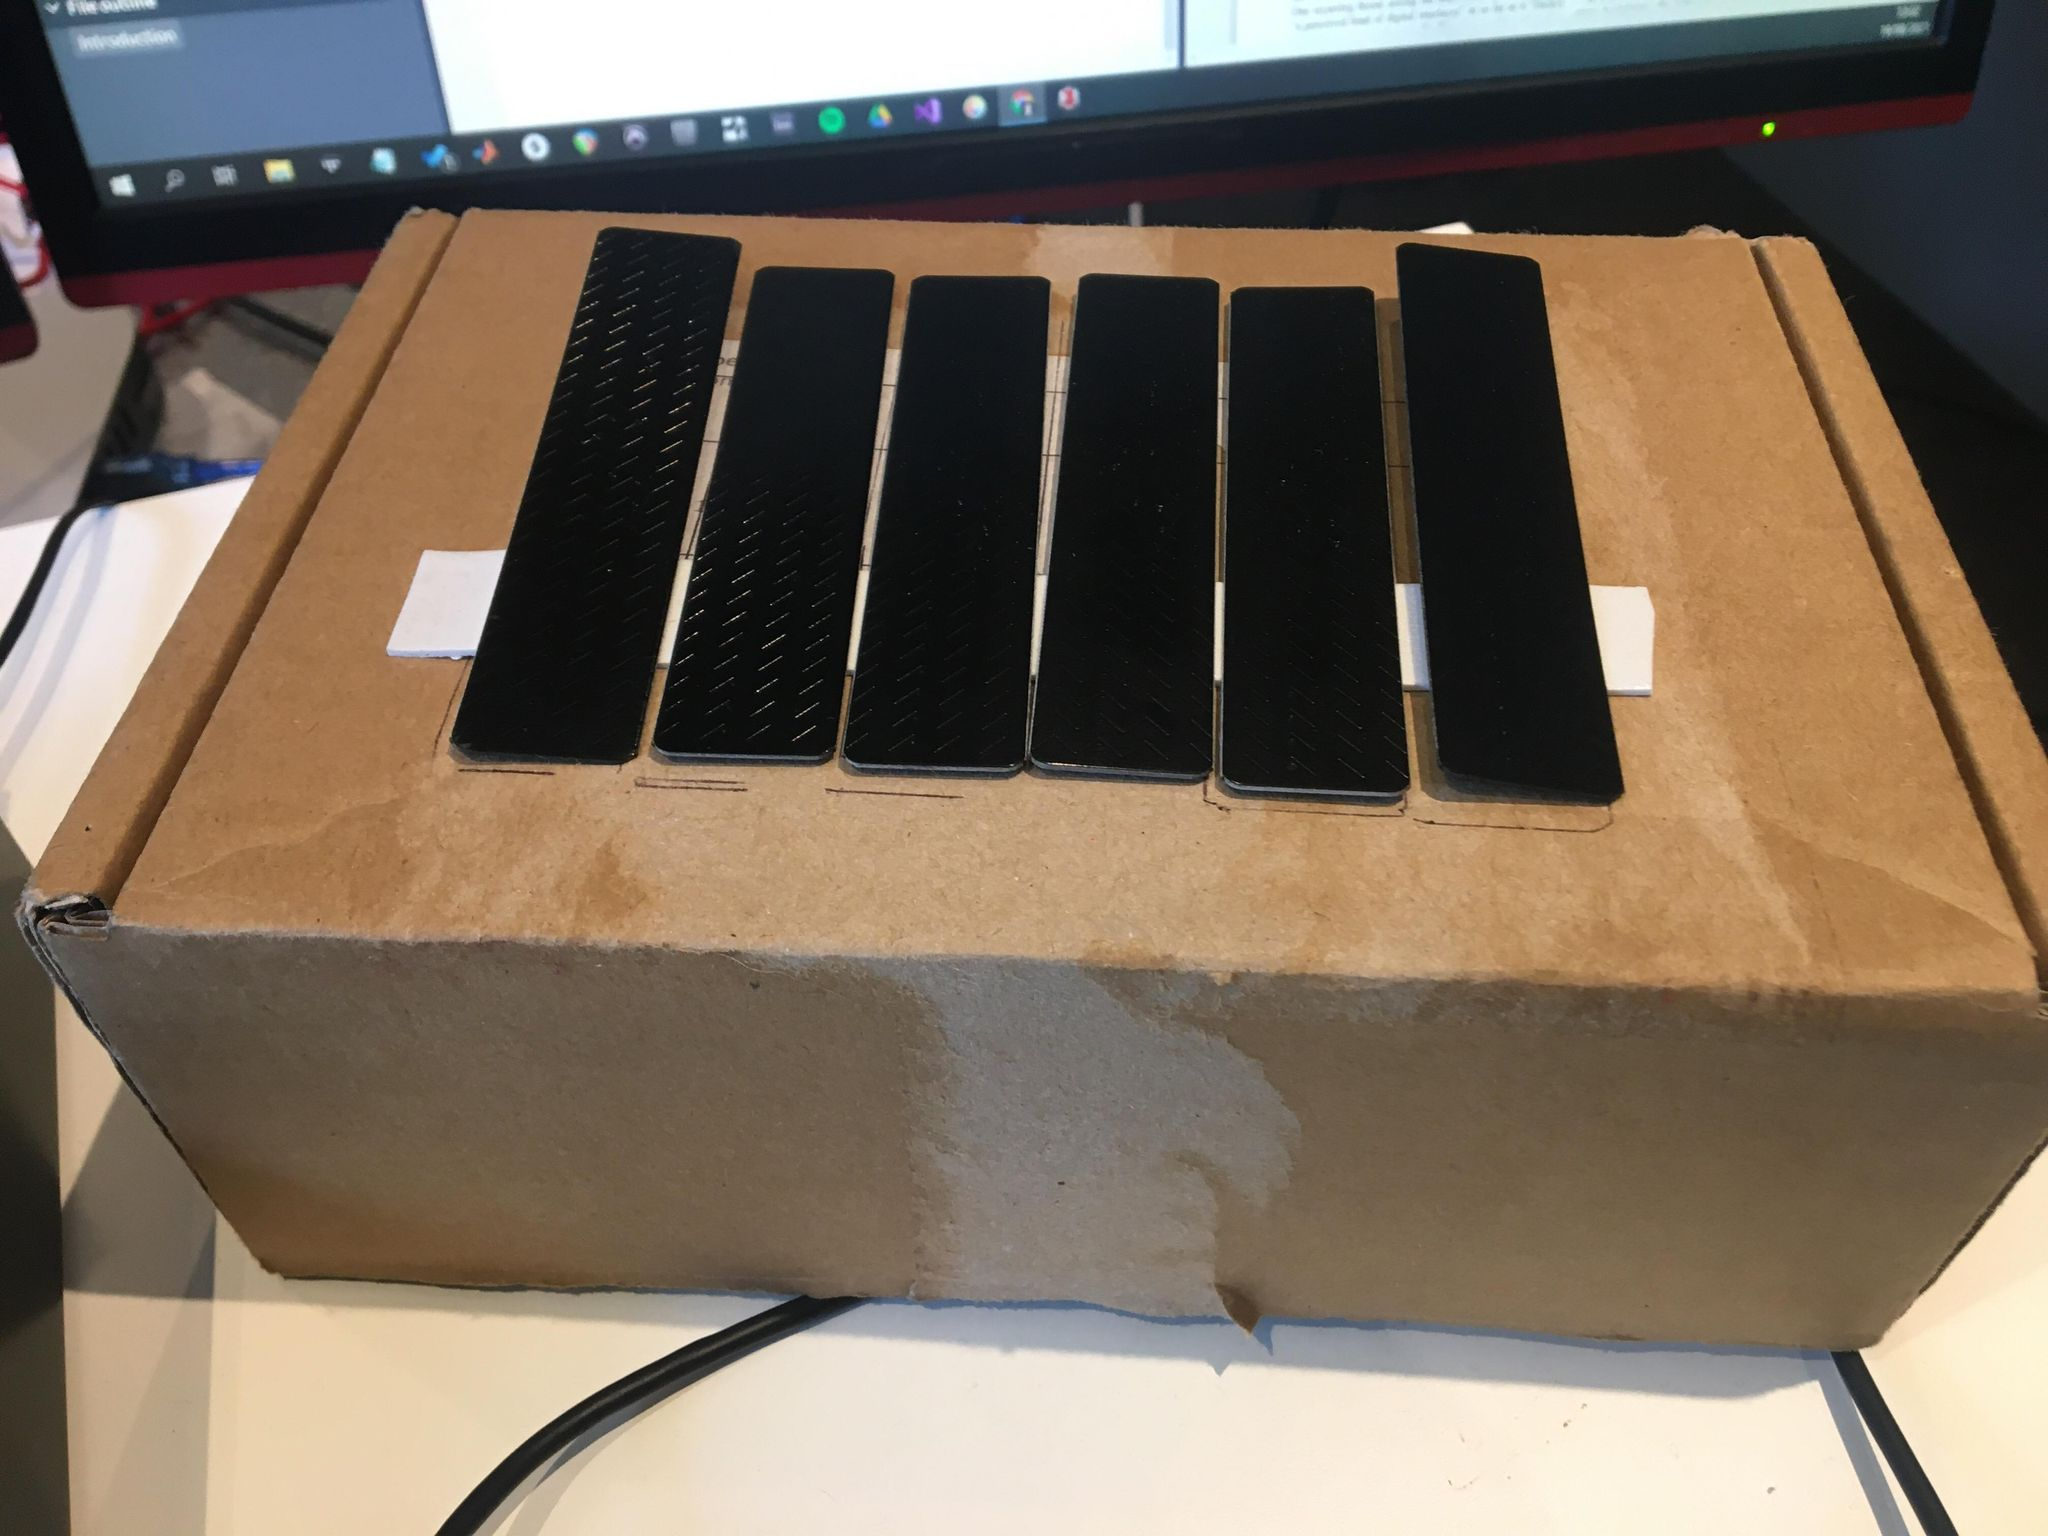
\includegraphics[scale=0.12]{Images/prototype.jpg}
    \caption{Basic proto-prototype.}
    \label{fig:protoprototype}
\end{figure}

This proto-prototype consisted of a small cardboard box that contained the main Bela, and a Trill Hub, with the Trill Bar sensors protruding from the top, which was sufficient to confirm that all the functionality was correct. 

\subsection{Choosing a guitar}
The width of string regions on a typical 6 string guitar is roughly 0.73cm. This may cause the width of each string zone to be quite small, and, at least, reduce the area for possible for pitch bends. This may also have presented a possible frustrating experience for the user, where it may have be to deliver precise finger movements.

Intention not mapping properly to outcome is likely to be frustrating for users. 

This is why, a seven string guitar was used as the basis for the prototype. Although, the prototype does fundamentally have a six string topology, the additional width per string allows for greater margin of error in finger placement. Although no direct comparison to a six-string has been made, this appears to help in the playablility of the prototype.

\subsection{Fitting the sensors}

To fit the sensors to the guitar required a few steps of minor carpentry. Because the Trill sensors have a substantial Grove connector on the rear as can be seen in Figure \ref{fig:trill_picture}. This meant that there had to be a hole cut on each of the frets that were to have sensors mounted. This was achieved by the use of a drill. 

Furthermore, the fret boards of typical guitars are not flat, and thus required sanding to accommodate the flat figure of the Trill sensors.

Additionally, the Trill sensors have their small chip protruding from the rear, which make mounting the sensors flush to the fret board difficult, so a corresponding area on each of the frets was extracted with a drill, such that each sensor was able to lie flush with the fret board. 